%%% Local Variables:
%%% coding: utf-8
%%% TeX-command-extra-options: "-shell-escape, -oytput-directory=build"
%%% End:

\documentclass[slidestop,compress,mathserif]{beamer}
\mode<presentation>
\beamertemplatenavigationsymbolsempty
\addtobeamertemplate{navigation symbols}{}{%
	\usebeamerfont{footline}%
	\usebeamercolor[fg]{footline}%
	\hspace{5em}%
	\textbf{\insertframenumber/\inserttotalframenumber}
}
\usepackage{minted}
\usepackage{latexsym}
\usepackage{menukeys}
\usepackage{bytefield}
\usepackage{textcomp}
\usepackage{varwidth}
\usepackage{naivemoha}

\usepackage{tikz}
\usetikzlibrary{shapes,arrows}

\usepackage{macro}

\usetheme{Antibes}
\usecolortheme{lily}

\AtBeginSubsection[]{
	\begin{frame}
	\vfill
	\centering
	\begin{beamercolorbox}[sep=8pt,center,shadow=true,rounded=true]{title}
		\insertsectionhead\newline\newline\usebeamerfont{title}\insertsubsectionhead\par%
	\end{beamercolorbox}
	\vfill
	\end{frame}
}

\title{VE482 Lab Notes}
\author{Yihao LIU, Hang SU, Yue YAO}
\institute{VE482 AU18 TA Group}
\begin{document}
\begin{frame} % Cover slide
	\titlepage
	\tiny{Source code available at https://github.com/tonyfloatersu/VE482-AU2018-LAB-NOTE}
\end{frame}

\begin{frame}[allowframebreaks]
    \small
    \frametitle{Table Of Contents}
    \tableofcontents
\end{frame}
\section{RC Week 7}
\subsection{Something about compilation}
\begin{frame}{What if we cannot distribute the source code?}
    \begin{block}{Examples of Absolute Dumb Solution}
		\begin{description}
        \item[Obfuscation] Nice try, but far from enough. A lot of code
            formatters are on their way.
        \item[Encryption] Decipher takes time, safety is not guaranteed, become
            useless if someone successfully cracked it.
        \item[Blabla ...] Don't really figure out any other dumb solutions.
        \end{description}
        \small{Good News: We don't have {\naive} solutions.}

        \small{Bad News: We don't have solutions. (Just joking, of course we have.)}
    \end{block}
\end{frame}

\begin{frame}[fragile]{Some example of obfuscation}
    \fontsize{3pt}{3pt}\selectfont
    \setbeamerfont{footnote}{size=\tiny}
    \begin{figure}[htp]
        \centering
        \RecustomVerbatimEnvironment{Verbatim}{BVerbatim}{}
        \inputminted{c}{code/week7/obfuscation.c}
    \end{figure}
    \let\thefootnote\relax\footnotetext{Source: https://www.ioccc.org/2015/yang/prog.c}
\end{frame}

\begin{frame}{Library is a current solution}
    \begin{block}{Definition}
        A pack of non-volatile code meant to be reused by the program.

        For C or C++ library, it comes in two parts:
        \begin{description}
        \item[Function Interface] A header file that exposes functionality of
            the library to whoever / whatever uses it.
        \item[Implementation] Pre-compiled binary file that contains machine
            code for source code implementation.
        \end{description}
    \end{block}

    \begin{block}{Tools Related}
        \begin{itemize}
        \item {Compiler}
        \item {Linker}
        \end{itemize}
    \end{block}
\end{frame}

\begin{frame}{Static / Dynamic}
    There are 2 types of library: static library and dynamic library.

    The biggest difference lies in the runtime of the target exec file.

    \begin{description}
    \item[Static Lib] The machine code is applied to target exec file, so the
        exec file do not need these static lib file in runtime.
    \item[Dynamic Lib] Target exec file still requires dynamic lib.
    \end{description}

    The different behavior lies in a fact that dynamic lib implementation is
    PIC, position-independent code.

    It can be executed / called regardless of absolute address in RAM.

\end{frame}

\begin{frame}{Static / Dynamic}
    \framesubtitle{Make such libraries}

    (For convenience and WLOG, we use \texttt{c++} and \texttt{g++} to
    illustrate.)

    \begin{block}{Static Lib}
        \begin{description}
        \item[Build lib] \texttt{g++ -c dumb.c}\\\texttt{ar rcs libdumb.a dumb.o}
        \item[Make exec] \texttt{g++ -o dumb main.c -L./ -ldumb}
        \end{description}
    \end{block}
    \begin{block}{Dynamic Lib}
        \begin{description}
        \item[Build lib] \texttt{g++ dumb.c -fPIC -shared -o libdumb.so}
        \item[Make exec] \texttt{g++ -o dumb main.c -L./ -ldumb}
        \end{description}
    \end{block}
\end{frame}

\begin{frame}{Experiment: size of executable file}
    \framesubtitle{Some knowledge you need to know}
    \begin{description}
    \item[Standalone Exec File]{The executable that doesn't require any
          external module / library / program. It is boot itself (bootstrap) and
          runs on bare ground of OS.}
    \item[Lib dependency detect]{\texttt{ldd} can find shared libraries of exec
          file.}
    \item[Lib linking order]{The order of lib linking should make a DAG
          directing the target source file. If inter-dependent situation
          happens, some fixes are needed.}
    \end{description}

\end{frame}

\begin{frame}{Experiment: size of executable file}
    \framesubtitle{Standalone Exec file}
    For \texttt{c++}, we use the following commandline parameters to make a
    standalone exec file:
    \newline\newline
    \texttt{-static -static-libgcc -static-libstdc++}
    \newline\newline
    These parameters guarantee that all the static version of dependencies are
    linked to the exec file.

\end{frame}

\begin{frame}[fragile]{Experiment: size of executable file}
    \framesubtitle{Lib dependency detect}

    An example of \texttt{ldd} usage:

    \inputminted[fontsize=\tiny]{shell-session}{code/week7/ldd_example.txt}

    Dependencies among dynamic libs exist. Here's another example:

    \inputminted[fontsize=\tiny]{shell-session}{code/week7/readelf_example.txt}

    Related commands like \texttt{objdump} can also be used.

    Better RTFM and use \texttt{man}.

\end{frame}

\begin{frame}{Experiment: size of executable file}
    \framesubtitle{Lib linking order (static acyclic)}
    \begin{columns}
        \column[]{.5\textwidth}
        \inputminted[fontsize=\tiny]{shell-session}{code/week7/static_acyclic.txt}
        \column[]{.5\textwidth}
        \inputminted[fontsize=\small]{shell-session}{code/week7/static_acyclic_dep.txt}
    \end{columns}
\end{frame}

\begin{frame}{Experiment: size of executable file}
    \framesubtitle{Lib linking order (dynamic acyclic)}
    \inputminted[fontsize=\tiny]{shell-session}{code/week7/dynamic_acyclic.txt}

    It can be noticed that \texttt{LD\_LIBRARY\_PATH} has been modified with
    current dir included, so dependency is automatically established.

    \inputminted[fontsize=\small]{shell-session}{code/week7/dynamic_acyclic_dep.txt}

\end{frame}

\begin{frame}{Experiment: size of executable file}
    \framesubtitle{Lib linking order (circular dependency)}
    \inputminted[fontsize=\small]{shell-session}{code/week7/circular.txt}
    The solution for static circular dependency is that:

    \texttt{gcc main.c -L. -lfo -lbar -lfo}
\end{frame}

\begin{frame}{Experiment: size of executable file}
    \framesubtitle{Experiment and Observes}
    \inputminted[fontsize=\tiny]{cpp}{code/week7/dumb.cpp}

    Then we get the following result:

    \inputminted[fontsize=\tiny]{shell-session}{code/week7/experiment_res.txt}
\end{frame}

\begin{frame}{Experiment: size of executable file}
    \framesubtitle{Analysis}
    \begin{block}{Dynamic Linking}
        \begin{itemize}
        \item Size: 18172
        \item \texttt{readelf -d ./dynamic\_dumb | grep 'NEEDED' | wc -l} is
            4. Indicating 4 shared libraries are used.
        \end{itemize}
    \end{block}
    \begin{block}{Static Standalone}
        \begin{itemize}
        \item Size: 2181936
        \item No shared library.
        \end{itemize}
    \end{block}
\end{frame}

\begin{frame}{Dependency Hell}
    \begin{block}{Dll Hell (Windows)}
        Problem arises when dll file version conflict between PC and program
        requirement. Dll file do not have the ability of backward compatibility,
        so minor changes in dll render internal structure different from
        previous version.
        \begin{figure}[htbp!]
            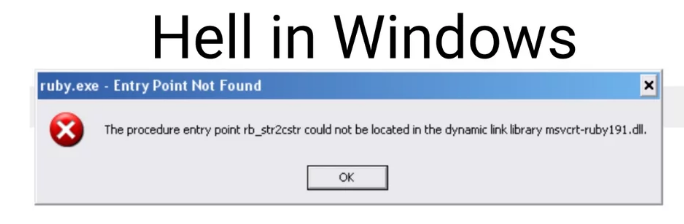
\includegraphics[width=10cm]{img/week7/dll_hell.png}
        \end{figure}
    \end{block}
\end{frame}

\begin{frame}{some meme}
    \begin{block}{Always be careful when creating libs!}
        \begin{figure}[htbp!]
            
\includegraphics[width=10cm]{img/week7/lib_meme.jpg}
        \end{figure}
        You can (not) redo.
    \end{block}
\end{frame}

\subsection{OK, what is multi-thread?}
\begin{frame}{Threads in Process}
\end{frame}
\subsection{Strategies about Multi-threading}
\subsection{\texttt{C++} Programming about Multi-threading}

\end{document}